\documentclass[12pt,answers]{book}
\usepackage{amsmath,amssymb}
\usepackage{geometry}
\geometry{
  letterpaper,
  total={170mm,257mm},
  left=20mm,
  right=20mm,
  top=30mm,  % Increase this value to make room for your header
  bottom=20mm,
  includeheadfoot  % This is crucial - it tells geometry to account for headers/footers
}
\usepackage{graphicx}
\usepackage{booktabs}
\usepackage{array}
\usepackage{multicol}

%\usepackage{hyperref}
\usepackage{tcolorbox}

\usepackage{listings}
\usepackage[usenames,dvipsnames]{xcolor}

\definecolor{codegreen}{rgb}{0,0.6,0}
\definecolor{codegray}{rgb}{0.5,0.5,0.5}
\definecolor{codepurple}{rgb}{0.58,0,0.82}
\definecolor{backcolour}{rgb}{0.96,0.96,0.96}
%\definecolor{backcolour}{rgb}{1,1,1}

\lstdefinestyle{mystyle}{
  backgroundcolor=\color{backcolour},
  commentstyle=\color{codegreen},
  keywordstyle=\color{magenta},
  numberstyle=\tiny\color{codegray},
  stringstyle=\color{codepurple},
  basicstyle=\ttfamily\footnotesize,
  breakatwhitespace=false,
  breaklines=true,
  captionpos=b,
  keepspaces=true,
  numbers=left,
  numbersep=5pt,
  showspaces=false,
  showstringspaces=false,
  showtabs=false,
  tabsize=2
}
\lstdefinelanguage{Julia}%
{morekeywords={abstract,break,case,catch,const,continue,do,else,elseif,%
    end,export,false,for,function,immutable,import,importall,if,in,%
    macro,module,otherwise,quote,return,switch,true,try,type,typealias,%
    using,while},%
  sensitive=true,%
  alsoother={$},%
  morecomment=[l]\#,%
  morecomment=[n]{\#=}{=\#},%
  morestring=[s]{"}{"},%
  morestring=[m]{'}{'},%
}[keywords,comments,strings]%

\lstset{%
  language         = Julia,
  basicstyle       = \ttfamily,
  keywordstyle     = \bfseries\color{blue},
  stringstyle      = \color{magenta},
  commentstyle     = \color{ForestGreen},
  showstringspaces = false,
}

\lstset{style=mystyle}

\makeatletter
\def\@makechapterhead#1{%
  \vspace*{-60pt}% Change this value to adjust vertical space before chapter heading
  {\parindent \z@ \raggedright \normalfont
    \ifnum \c@secnumdepth >\m@ne
    \huge\bfseries \@chapapp\space \thechapter
    \par\nobreak
    \vskip 20\p@
    \fi
    \interlinepenalty\@M
    \Huge \bfseries #1\par\nobreak
    \vskip 40\p@
}}
\makeatother

\usepackage{fancyhdr,lastpage}
\pagestyle{fancy}
\fancyhead[L]{\textbf{Spring 2025}}
\fancyhead[R]{\textbf{Student:}\hspace{5cm}}
\fancyhead[C]{}
\fancyfoot[L]{MTH229 Calculus Laboratory Notebook}
\fancyfoot[C]{}
\fancyfoot[R]{Page \thepage\ of \pageref{LastPage}}
\renewcommand{\headrulewidth}{2pt}
\renewcommand{\footrulewidth}{2pt}

%\newcommand{\eb}[1]{\begin{tcolorbox}[width=0.90\textwidth, height={#1}cm] ~ \end{tcolorbox}}


\newcommand{\eb}{\begin{tcolorbox}[width=0.90\textwidth, height=4cm, colback=white]
    ~
  \end{tcolorbox}}

\newcommand{\ebb}{\begin{tcolorbox}[width=0.90\textwidth, height=9cm, colback=white]
    ~
  \end{tcolorbox}}

\newcommand{\ebbb}{\begin{tcolorbox}[width=0.90\textwidth, height=2cm, colback=white]
    ~
    \end{tcolorbox}}

\newcommand{\ebbbb}{\begin{tcolorbox}[width=0.90\textwidth, height=1cm, colback=white]
    ~
    \end{tcolorbox}}




\title{MTH229 Notes}
\date{Spring 2025}
\author{Professor Kevin O'Bryant}

\newcommand{\julia}{{\tt Julia}}

\begin{document}

  \maketitle
\chapter*{First Day Checklist}
Lab Rules: Attendance is required, each and every lab period for the full lab period. You are not to use a phone in the lab for texting, calling, nor browsing. No goofing off, that is.

\noindent {\bf Checklist for the bare minimum first day work.}
\begin{description}
  \item[$\square$] Log into the campus network SLAS.
  \item[$\square$] Log into Brightspace and see if there are any announcements for this lab class.
  \item[$\square$] Make sure the email address that Brightspace has is one that works for you.
  \item[$\square$] Make sure the email address that CUNYFirst has for you is one that you monitor.
  \item[$\square$] Take a look at the Syllabus, also located on Brightspace.
  \item[$\square$] WeBWorK is the service that we will use to assign and grade homework. Log in to WeBWorK at \\ \verb|https://www.math.csi.cuny.edu/webwork2/| and selecting your professor's name
  or by going to the math department website \verb|https://www.math.csi.cuny.edu/|, finding the ``WeBWorK'' link at the lower right, and then selecting our class. You will find your username and initial password described on that page (it is your first initial, last name, and 4 digits from ID). If it doesn't work, your professor can help.
  \item[$\square$] Change WeBWorK password. WeBWorK is not secure: you should not re-use a password from a system you care about. It's under ``User Settings'', as is an email address that will be used by WeBWorK. Change it, too, if you want. Course related emails will go through the CUNYFirst address or the Brightspace address, but exchanges about specific homework problems will go through WeBWorK. If you ever forget your password, your professor can reset it.
  \item[$\square$] Contact someone else in the classroom by sending them a chat message, or a text, or just using your old-fashioned voice. Say hello, exchange email addresses, etc. It's okay to do this with several people.
  \item[$\square$] Open ``Problem 1'' of the first homework set, ``01-calculator''.
  \item[$\square$] Use the ``Juliabox'' button at the top of the problem. Your login name and Juliabox password are both set to your WeBWorK username. It works best if you are using Chrome.
  \item[$\square$] Open the ``01-calculator.ipynb'' file. This opens our textbook. Read through this material. The first line is ``Read about this material here'' with a link. That link will take you to a \emph{more} detailed and in-depth explanation --- I advise you to skip it at least until you are stuck on a problem. After giving this material a read-through, you will come to a blank input line at the bottom. Look at the WeBWorK problem. Try to do it in the blank input line at the bottom. If you can't, get in touch with your instructor.
  \item[$\square$] When you have the value for (a), copy-and-paste it into the WeBWorK blank. Press the ``Submit Answers'' button at the bottom of the WeBWorK page. This saves your answer, and also tells you if it was correct or incorrect. You have unlimited attempts for most problems, including this one.
  \item[$\square$] You are expected to do your own work, but you are not expected to do it alone. The best experience for this class is to work in parallel with someone, as it helps to have someone to bounce ideas around and have fresh eyes, occasionally. Do not split the work in half: everyone needs to do and understand every problem. There's plenty of time.
  \item[$\square$] You should do several problems from this project on the first day. Some people are able to finish it, even. It should definitely be completed by (at the latest) the end of the second lab period. Note that the due dates shown in WeBWorK are deadlines: they will not be postponed under (almost) any circumstances. You are expected to finish the projects a week or more \emph{ahead} of the deadlines.
  \item[$\square$] At the end of lab period, navigate to the first problem that you have not completed (or the last problem, if you've completed them all), and press the ``email instructor'' button. In the message, include the names of the people sitting next to you. This email will count as your attendance at the first lab period.
\end{description}

\chapter*{Installing \julia}

It is in principle easy to install \julia on any computer, including laptops. This is sometimes broken, as there are too many types of computers with too many possible combinations of software on them.

The best advice I can give is to check out \verb|www.julialang.org| and download the version that seems most appropriate for your situation.


\chapter{01-calculator}

\begin{enumerate}
  \item Problem 1: \hspace{2cm} Title: \underline{``Using {\tt Julia} like a calculator''}
  \begin{enumerate}
  \item Summary of the problem:
    \begin{tcolorbox}[height=2cm]
           evaluating simple expressions \vspace{1cm}
    \end{tcolorbox}
     \item What I was supposed to learn:
     \begin{tcolorbox}[height=5cm]
      adding, subtracting, multiplying in {\tt Julia}
      \vspace{1cm}

      When I want to multiply, I should use \textasteriskcentered\vspace{1cm}

      I should put parentheses around numerators and denominators if they have more than one term.
    \end{tcolorbox}

  \item Date started, finished, and time spent
    \begin{tcolorbox}[height=1cm]
          started 25-2-27, finished 25-2-27, 10 minutes\vspace{1cm}
    \end{tcolorbox}


  \item Difficulty:
    \begin{tcolorbox}[height=1cm]
      1 out of 10
    \end{tcolorbox}

  \end{enumerate}

\clearpage
\item Problem 2: \hspace{2cm} Title: \underline{``Precedence (PEMDAS)''}
  \begin{enumerate}
  \item Summary of the problem \eb
  \item What I was supposed to learn \ebb
  \item Date started, finished, and time spent \ebbb
  \item Difficulty: \ebbbb
  \end{enumerate}

\clearpage

\item Problem 3: \hspace{2cm} Title: \underline{\hspace{8cm}}
\begin{enumerate}
\item Summary of the problem \eb
\item What I was supposed to learn \ebb
\item Date started, finished, and time spent \ebbb
\item Difficulty: \ebbbb
\end{enumerate}
\clearpage

  \item Problem 4: \hspace{2cm} Title: \underline{\hspace{8cm}}
\begin{enumerate}
\item Summary of the problem \eb
\item What I was supposed to learn \ebb
\item Date started, finished, and time spent \ebbb
\item Difficulty: \ebbbb
\end{enumerate}

\clearpage

  \item Problem 5: \hspace{2cm} Title: \underline{\hspace{8cm}}
\begin{enumerate}
\item Summary of the problem \eb
\item What I was supposed to learn \ebb
\item Date started, finished, and time spent \ebbb
\item Difficulty: \ebbbb
\end{enumerate}

\clearpage

  \item Problem 6: \hspace{2cm} Title: \underline{\hspace{8cm}}
\begin{enumerate}
\item Summary of the problem \eb
\item What I was supposed to learn \ebb
\item Date started, finished, and time spent \ebbb
\item Difficulty: \ebbbb
\end{enumerate}
\clearpage
  \item Problem 7: \hspace{2cm} Title: \underline{\hspace{8cm}}
\begin{enumerate}
\item Summary of the problem \eb
\item What I was supposed to learn \ebb
\item Date started, finished, and time spent \ebbb
\item Difficulty: \ebbbb
\end{enumerate}
\clearpage
  \item Problem 8: \hspace{2cm} Title: \underline{\hspace{8cm}}
\begin{enumerate}
\item Summary of the problem \eb
\item What I was supposed to learn \ebb
\item Date started, finished, and time spent \ebbb
\item Difficulty: \ebbbb
\end{enumerate}

\end{enumerate}

\clearpage

\chapter{02-functions}

Define the function $$f(x) = \frac{(x-1)^2}{x^2+3x+2} + \tan^{-1}(x) + \frac{1}{\sqrt{2\pi}}e^{-x^2/2}$$
and use your function to find $f(0), f(1), f(-3/2)$.

\vspace{1cm}
\noindent {\bf Solution:}
We input the following:
\begin{lstlisting}[language=Julia]
f(x) = (x-1)^2 / (x^2+3x+2) + atan(x) + 1/sqrt(2*pi)*exp(-x^2/2)
f(0),f(1),f(-3/2)
\end{lstlisting}
and the output is the following:
\begin{lstlisting}[language=Julia]
(0.8989422804014326, 1.0273688879165916, -25.853276127581438)
\end{lstlisting}
Thus,
\begin{align*}
  f(0) &\approx 0.8989422804014326\\
  f(1) &\approx 1.0273688879165916\\
  f(-3/2) &\approx -25.853276127581438\\
\end{align*}

\clearpage
\begin{enumerate}
\item Problem 1: \hspace{2cm} Title: \underline{\hspace{8cm}}
\begin{enumerate}
  \item Summary of the problem \eb
  \item What I was supposed to learn \ebb
  \item Date started, finished, and time spent \ebbb
  \item Difficulty: \ebbbb
\end{enumerate}
\item Problem 2: \hspace{2cm} Title: \underline{\hspace{8cm}}
\begin{enumerate}
  \item Summary of the problem \eb
  \item What I was supposed to learn \ebb
  \item Date started, finished, and time spent \ebbb
  \item Difficulty: \ebbbb
\end{enumerate}

\clearpage
\item Problem 3: \hspace{2cm} Title: \underline{\hspace{8cm}}
\begin{enumerate}
  \item Summary of the problem \eb
  \item What I was supposed to learn \ebb
  \item Date started, finished, and time spent \ebbb
  \item Difficulty: \ebbbb
\end{enumerate}
\clearpage
\item Problem 4: \hspace{2cm} Title: \underline{\hspace{8cm}}
\begin{enumerate}
  \item Summary of the problem \eb
  \item What I was supposed to learn \ebb
  \item Date started, finished, and time spent \ebbb
  \item Difficulty: \ebbbb
\end{enumerate}
\clearpage
\item Problem 5: \hspace{2cm} Title: \underline{\hspace{8cm}}
\begin{enumerate}
  \item Summary of the problem \eb
  \item What I was supposed to learn \ebb
  \item Date started, finished, and time spent \ebbb
  \item Difficulty: \ebbbb
\end{enumerate}
\clearpage
\item Problem 6: \hspace{2cm} Title: \underline{\hspace{8cm}}
\begin{enumerate}
  \item Summary of the problem \eb
  \item What I was supposed to learn \ebb
  \item Date started, finished, and time spent \ebbb
  \item Difficulty: \ebbbb
\end{enumerate}
\end{enumerate}

\clearpage

\chapter{03-graphics}

Make a plot of the periodic function $\displaystyle f(x)=\sin(9\cos(2\sin(\frac{\pi x}{2})))$ over one period.

\vspace{5mm}
\noindent {\bf Solution:}
We input the code on the left and are rewarded with the picture on the right.\newline
\begin{minipage}[b]{0.49\textwidth}
\begin{lstlisting}[language=Julia]
using MTH229, Plots
f(x) = sin(9*cos(2*sin(pi*x/2)))
plot(f,-10,10)
\end{lstlisting}
\end{minipage}
\begin{minipage}{0.49\textwidth}
  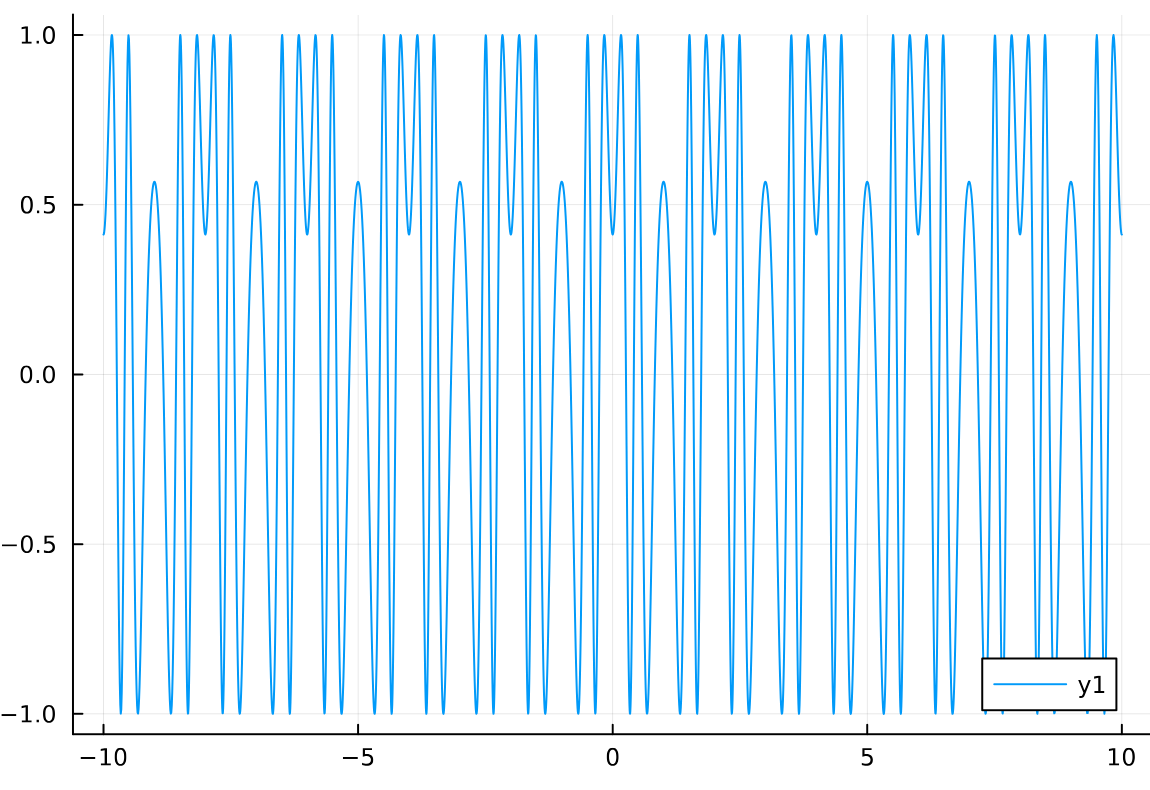
\includegraphics[width=0.7\linewidth]{SkeletonNotes/03-graphics-1}
\end{minipage}\newline
From that image, we count 9 or 10 periods. We decide to look at the graph over the domain $[0,5]$
\begin{minipage}[b]{0.49\textwidth}
  \begin{lstlisting}[language=Julia]
plot(f,0,5)
  \end{lstlisting}
\end{minipage}
\begin{minipage}{0.49\textwidth}
  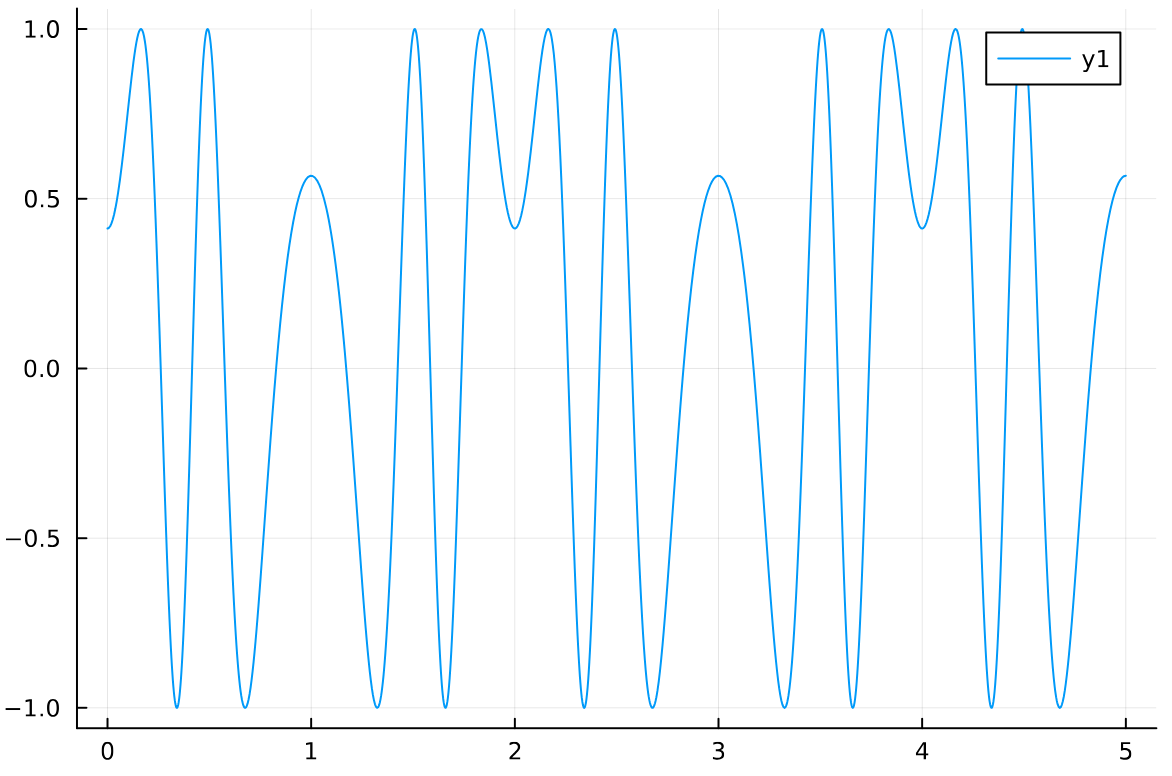
\includegraphics[width=0.7\linewidth]{SkeletonNotes/03-graphics-2}
\end{minipage}\newline
We graphically conclude that the period is 2, and make the required graph.\newline
\begin{minipage}[b]{0.49\textwidth}
  \begin{lstlisting}[language=Julia]
plot(f,0,2)
  \end{lstlisting}
\end{minipage}
\begin{minipage}{0.49\textwidth}
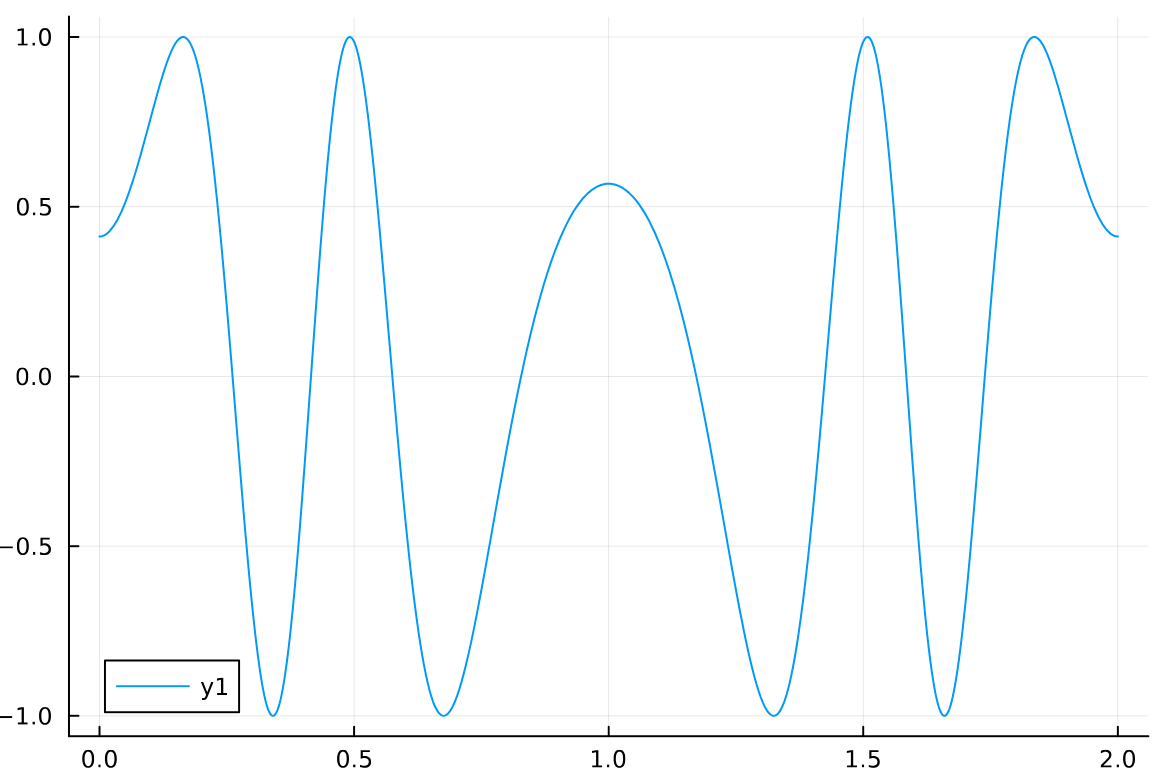
\includegraphics[width=0.7\linewidth]{SkeletonNotes/03-graphics-3}
\end{minipage}



\clearpage
\begin{enumerate}
  \item Problem 1: \hspace{2cm} Title: \underline{\hspace{8cm}}
  \begin{enumerate}
    \item Summary of the problem \eb
    \item What I was supposed to learn \ebb
    \item Date started, finished, and time spent \ebbb
    \item Difficulty: \ebbbb
  \end{enumerate}
  \item Problem 2: \hspace{2cm} Title: \underline{\hspace{8cm}}
  \begin{enumerate}
    \item Summary of the problem \eb
    \item What I was supposed to learn \ebb
    \item Date started, finished, and time spent \ebbb
    \item Difficulty: \ebbbb
  \end{enumerate}
  \clearpage
  \item Problem 3: \hspace{2cm} Title: \underline{\hspace{8cm}}
  \begin{enumerate}
    \item Summary of the problem \eb
    \item What I was supposed to learn \ebb
    \item Date started, finished, and time spent \ebbb
    \item Difficulty: \ebbbb
  \end{enumerate}
  \clearpage
  \item Problem 4: \hspace{2cm} Title: \underline{\hspace{8cm}}
  \begin{enumerate}
    \item Summary of the problem \eb
    \item What I was supposed to learn \ebb
    \item Date started, finished, and time spent \ebbb
    \item Difficulty: \ebbbb
  \end{enumerate}
  \clearpage
  \item Problem 5: \hspace{2cm} Title: \underline{\hspace{8cm}}
  \begin{enumerate}
    \item Summary of the problem \eb
    \item What I was supposed to learn \ebb
    \item Date started, finished, and time spent \ebbb
    \item Difficulty: \ebbbb
  \end{enumerate}
  \clearpage
  \item Problem 6: \hspace{2cm} Title: \underline{\hspace{8cm}}
  \begin{enumerate}
    \item Summary of the problem \eb
    \item What I was supposed to learn \ebb
    \item Date started, finished, and time spent \ebbb
    \item Difficulty: \ebbbb
  \end{enumerate}
  \clearpage
  \item Problem 7: \hspace{2cm} Title: \underline{\hspace{8cm}}
  \begin{enumerate}
    \item Summary of the problem \eb
    \item What I was supposed to learn \ebb
    \item Date started, finished, and time spent \ebbb
    \item Difficulty: \ebbbb
  \end{enumerate}
\end{enumerate}

\clearpage

\chapter{04-zeros}
Solve the equation $\displaystyle \exp(7+\sin x) = 2x^2+2x+9.$

\vspace{5mm}
\noindent {\bf Solution:}
First, we define the functions and plot them together.\newline
\begin{minipage}{0.49\textwidth}
\begin{lstlisting}[language=Julia]
using MTH229, Plots
left(x) = exp(7+sin(x))
right(x) = 2x^2 + 2x + 9
plot(left, -10, 10)
plot!(right)
\end{lstlisting}
\end{minipage}
\begin{minipage}{0.49\textwidth}
  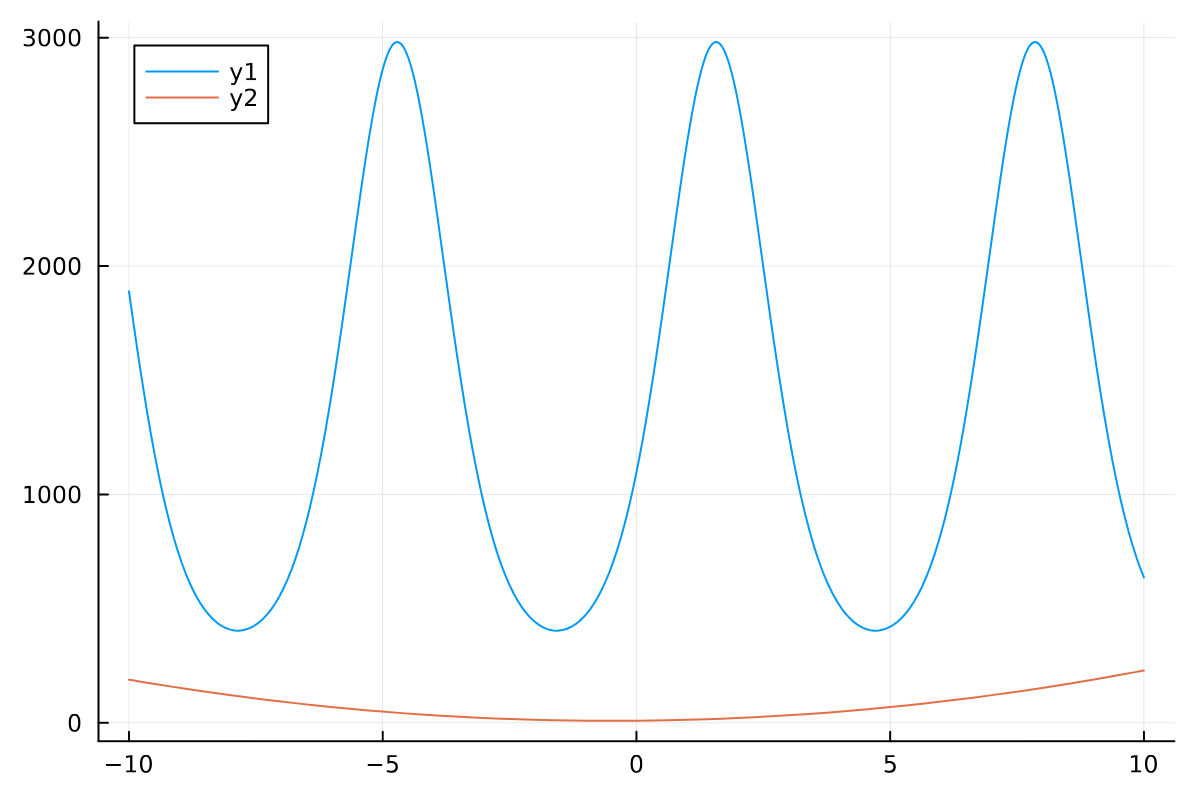
\includegraphics[width=0.7\linewidth]{SkeletonNotes/04-graphics-1}
\end{minipage}\newline
We think: As $-1\le \sin x \le 1$, it must be that $e^6 \le \exp(7+\sin x) \le e^8$. Also, we know that $y=2x^2+2x+9$ is a parabola. We visualize it arcing up to where it crosses above $y=e^8$. With that in mind, we make a picture over $[-100,100]$, and from that picture decide to instead use $[-50,50]$. From that picture, we decide to use $[-40,40]$.\newline
\begin{minipage}{0.49\textwidth}
\begin{lstlisting}[language=Julia]
plot(left, -40, 40)
plot!(right)
\end{lstlisting}
\end{minipage}
\begin{minipage}{0.49\textwidth}
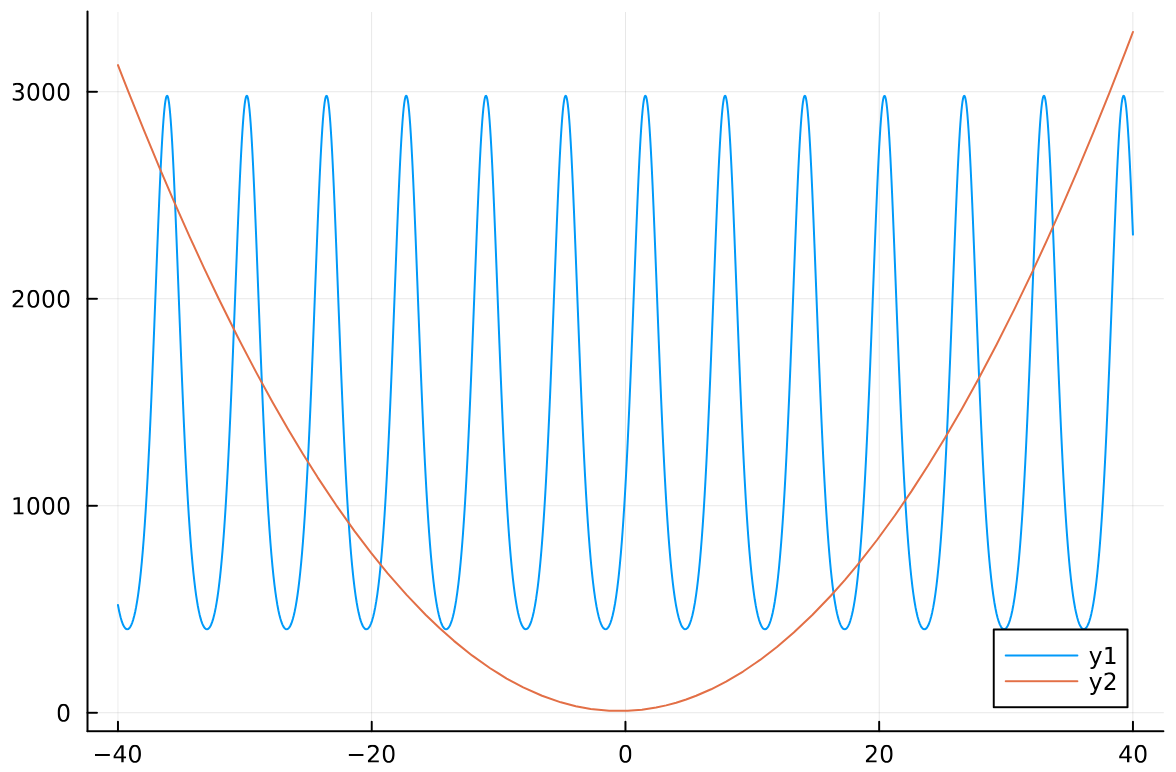
\includegraphics[width=0.7\linewidth]{SkeletonNotes/04-graphics-2}
\end{minipage}\newline
Now we can see 14 solutions, and there's a close call around $x\approx-16$ that we can't see visually if the graphs intersect or not. Now, we can use {\tt fzeros} to find the solutions.
\begin{lstlisting}[language=Julia]
aux(x) = left(x) - right(x)
fzeros(aux, -40, 40)
\end{lstlisting}
The output is a list of all 14 solutions. There is no solution close to $-16$, which we double-check by plotting over the domain $[-18,-13]$.

\clearpage

\begin{enumerate}
  \item Problem 1: \hspace{2cm} Title: \underline{\hspace{8cm}}
  \begin{enumerate}
    \item Summary of the problem \eb
    \item What I was supposed to learn \ebb
    \item Date started, finished, and time spent \ebbb
    \item Difficulty: \ebbbb
  \end{enumerate}
  \item Problem 2: \hspace{2cm} Title: \underline{\hspace{8cm}}
  \begin{enumerate}
    \item Summary of the problem \eb
    \item What I was supposed to learn \ebb
    \item Date started, finished, and time spent \ebbb
    \item Difficulty: \ebbbb
  \end{enumerate}
  \clearpage
  \item Problem 3: \hspace{2cm} Title: \underline{\hspace{8cm}}
  \begin{enumerate}
    \item Summary of the problem \eb
    \item What I was supposed to learn \ebb
    \item Date started, finished, and time spent \ebbb
    \item Difficulty: \ebbbb
  \end{enumerate}
  \clearpage
  \item Problem 4: \hspace{2cm} Title: \underline{\hspace{8cm}}
  \begin{enumerate}
    \item Summary of the problem \eb
    \item What I was supposed to learn \ebb
    \item Date started, finished, and time spent \ebbb
    \item Difficulty: \ebbbb
  \end{enumerate}
  \clearpage
  \item Problem 5: \hspace{2cm} Title: \underline{\hspace{8cm}}
  \begin{enumerate}
    \item Summary of the problem \eb
    \item What I was supposed to learn \ebb
    \item Date started, finished, and time spent \ebbb
    \item Difficulty: \ebbbb
  \end{enumerate}
  \clearpage
  \item Problem 6: \hspace{2cm} Title: \underline{\hspace{8cm}}
  \begin{enumerate}
    \item Summary of the problem \eb
    \item What I was supposed to learn \ebb
    \item Date started, finished, and time spent \ebbb
    \item Difficulty: \ebbbb
  \end{enumerate}
\end{enumerate}

\clearpage

\chapter{05-limits}
Compute $\displaystyle \lim_{x\to 0} \frac{\tan (x) (\sin (x)-\cos (x)-1)}{\exp (x)-1}$ three different ways.

\vspace{5mm}
\noindent {\bf Solution:}
First, we define a function, and then we plot it on an interval around 0 (because it is a limit as $x\to0$):\newline
\begin{minipage}{0.49\textwidth}
\begin{lstlisting}[language=Julia]
using MTH229, Plots
top(x) = tan(x) * (sin(x)-cos(x)-1)
bot(x) = exp(x) -1
f(x) = top(x) / bot(x)
plot(f, -0.5, 0.5 )
\end{lstlisting}
\end{minipage}
\begin{minipage}{0.49\textwidth}
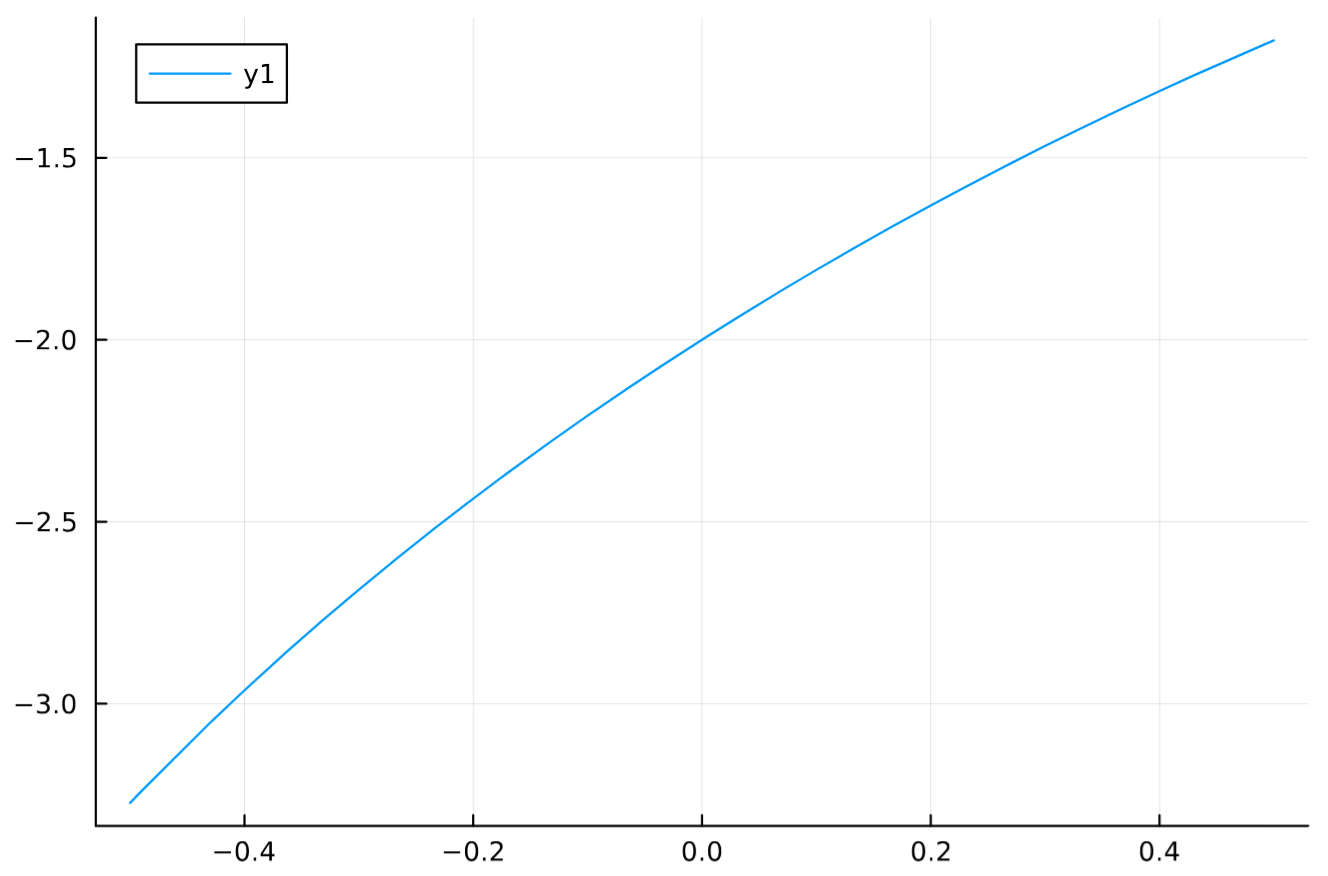
\includegraphics[width=0.7\linewidth]{SkeletonNotes/05-graphics-1}
\end{minipage}\newline
From the image, we conclude that the limit is about $-2$.

Alternatively, we could make a table showing inputs getting close to 0 and see what the outputs are getting close to.\newline
\begin{minipage}{0.45\textwidth}
  \begin{lstlisting}[language=Julia]
    lim(f, 0 )
  \end{lstlisting}
\end{minipage}
\begin{minipage}{0.49\textwidth}
  \centering
  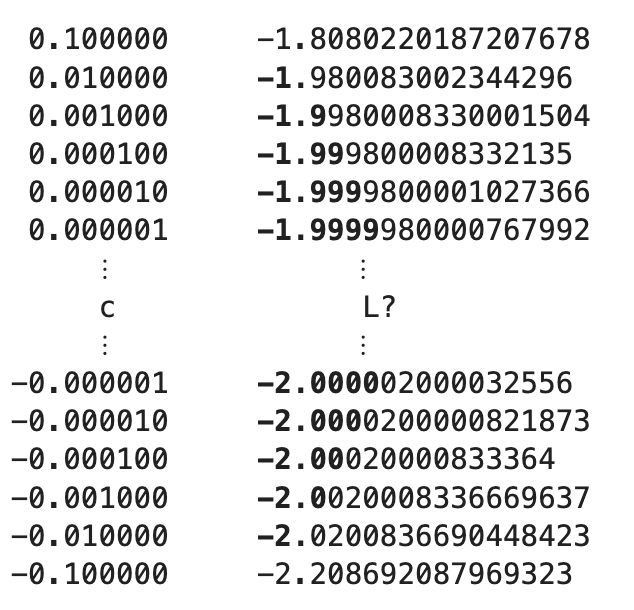
\includegraphics[width=0.6\linewidth]{SkeletonNotes/05-graphics-2}
\end{minipage}\newline
We see in the second column that $L$ wants to be $-2$.

Alternatively, we could use {\tt SymPy}, which is loaded with the {\tt MTH229} package.\newline
\begin{lstlisting}[language=Julia]
@syms x
limit(f(x), x => 0 )
\end{lstlisting}
which outputs a simple ``$-2$''.

\clearpage
\begin{enumerate}
  \item Problem 1: \hspace{2cm} Title: \underline{\hspace{8cm}}
  \begin{enumerate}
    \item Summary of the problem \eb
    \item What I was supposed to learn \ebb
    \item Date started, finished, and time spent \ebbb
    \item Difficulty: \ebbbb
  \end{enumerate}
  \item Problem 2: \hspace{2cm} Title: \underline{\hspace{8cm}}
  \begin{enumerate}
    \item Summary of the problem \eb
    \item What I was supposed to learn \ebb
    \item Date started, finished, and time spent \ebbb
    \item Difficulty: \ebbbb
  \end{enumerate}
  \clearpage
  \item Problem 3: \hspace{2cm} Title: \underline{\hspace{8cm}}
  \begin{enumerate}
    \item Summary of the problem \eb
    \item What I was supposed to learn \ebb
    \item Date started, finished, and time spent \ebbb
    \item Difficulty: \ebbbb
  \end{enumerate}
  \clearpage
  \item Problem 4: \hspace{2cm} Title: \underline{\hspace{8cm}}
  \begin{enumerate}
    \item Summary of the problem \eb
    \item What I was supposed to learn \ebb
    \item Date started, finished, and time spent \ebbb
    \item Difficulty: \ebbbb
  \end{enumerate}
  \clearpage
  \item Problem 5: \hspace{2cm} Title: \underline{\hspace{8cm}}
  \begin{enumerate}
    \item Summary of the problem \eb
    \item What I was supposed to learn \ebb
    \item Date started, finished, and time spent \ebbb
    \item Difficulty: \ebbbb
  \end{enumerate}
  \clearpage
  \item Problem 6: \hspace{2cm} Title: \underline{\hspace{8cm}}
  \begin{enumerate}
    \item Summary of the problem \eb
    \item What I was supposed to learn \ebb
    \item Date started, finished, and time spent \ebbb
    \item Difficulty: \ebbbb
  \end{enumerate}
\end{enumerate}

\clearpage

\chapter{06-derivatives}\clearpage
\begin{enumerate}
  \item Problem 1: \hspace{2cm} Title: \underline{\hspace{8cm}}
  \begin{enumerate}
    \item Summary of the problem \eb
    \item What I was supposed to learn \ebb
    \item Date started, finished, and time spent \ebbb
    \item Difficulty: \ebbbb
  \end{enumerate}
  \item Problem 2: \hspace{2cm} Title: \underline{\hspace{8cm}}
  \begin{enumerate}
    \item Summary of the problem \eb
    \item What I was supposed to learn \ebb
    \item Date started, finished, and time spent \ebbb
    \item Difficulty: \ebbbb
  \end{enumerate}

  \clearpage
  \item Problem 3: \hspace{2cm} Title: \underline{\hspace{8cm}}
  \begin{enumerate}
    \item Summary of the problem \eb
    \item What I was supposed to learn \ebb
    \item Date started, finished, and time spent \ebbb
    \item Difficulty: \ebbbb
  \end{enumerate}
  \clearpage
  \item Problem 4: \hspace{2cm} Title: \underline{\hspace{8cm}}
  \begin{enumerate}
    \item Summary of the problem \eb
    \item What I was supposed to learn \ebb
    \item Date started, finished, and time spent \ebbb
    \item Difficulty: \ebbbb
  \end{enumerate}
  \clearpage
  \item Problem 5: \hspace{2cm} Title: \underline{\hspace{8cm}}
  \begin{enumerate}
    \item Summary of the problem \eb
    \item What I was supposed to learn \ebb
    \item Date started, finished, and time spent \ebbb
    \item Difficulty: \ebbbb
  \end{enumerate}
  \clearpage
  \item Problem 6: \hspace{2cm} Title: \underline{\hspace{8cm}}
  \begin{enumerate}
    \item Summary of the problem \eb
    \item What I was supposed to learn \ebb
    \item Date started, finished, and time spent \ebbb
    \item Difficulty: \ebbbb
  \end{enumerate}
  \clearpage
  \item Problem 7: \hspace{2cm} Title: \underline{\hspace{8cm}}
  \begin{enumerate}
    \item Summary of the problem \eb
    \item What I was supposed to learn \ebb
    \item Date started, finished, and time spent \ebbb
    \item Difficulty: \ebbbb
  \end{enumerate}
  \clearpage
  \item Problem 8: \hspace{2cm} Title: \underline{\hspace{8cm}}
  \begin{enumerate}
    \item Summary of the problem \eb
    \item What I was supposed to learn \ebb
    \item Date started, finished, and time spent \ebbb
    \item Difficulty: \ebbbb
  \end{enumerate}
  \clearpage
  \item Problem 9: \hspace{2cm} Title: \underline{\hspace{8cm}}
  \begin{enumerate}
    \item Summary of the problem \eb
    \item What I was supposed to learn \ebb
    \item Date started, finished, and time spent \ebbb
    \item Difficulty: \ebbbb
  \end{enumerate}
\end{enumerate}

\clearpage

\chapter{07-newton}\clearpage
\begin{enumerate}
  \item Problem 1: \hspace{2cm} Title: \underline{\hspace{8cm}}
  \begin{enumerate}
    \item Summary of the problem \eb
    \item What I was supposed to learn \ebb
    \item Date started, finished, and time spent \ebbb
    \item Difficulty: \ebbbb
  \end{enumerate}
  \item Problem 2: \hspace{2cm} Title: \underline{\hspace{8cm}}
  \begin{enumerate}
    \item Summary of the problem \eb
    \item What I was supposed to learn \ebb
    \item Date started, finished, and time spent \ebbb
    \item Difficulty: \ebbbb
  \end{enumerate}
  \clearpage
  \item Problem 3: \hspace{2cm} Title: \underline{\hspace{8cm}}
  \begin{enumerate}
    \item Summary of the problem \eb
    \item What I was supposed to learn \ebb
    \item Date started, finished, and time spent \ebbb
    \item Difficulty: \ebbbb
  \end{enumerate}
  \clearpage
  \item Problem 4: \hspace{2cm} Title: \underline{\hspace{8cm}}
  \begin{enumerate}
    \item Summary of the problem \eb
    \item What I was supposed to learn \ebb
    \item Date started, finished, and time spent \ebbb
    \item Difficulty: \ebbbb
  \end{enumerate}
  \clearpage
  \item Problem 5: \hspace{2cm} Title: \underline{\hspace{8cm}}
  \begin{enumerate}
    \item Summary of the problem \eb
    \item What I was supposed to learn \ebb
    \item Date started, finished, and time spent \ebbb
    \item Difficulty: \ebbbb
  \end{enumerate}
  \clearpage
  \item Problem 6: \hspace{2cm} Title: \underline{\hspace{8cm}}
  \begin{enumerate}
    \item Summary of the problem \eb
    \item What I was supposed to learn \ebb
    \item Date started, finished, and time spent \ebbb
    \item Difficulty: \ebbbb
  \end{enumerate}
\end{enumerate}

\clearpage

\chapter{08-first second derivatives}\clearpage
\begin{enumerate}
  \item Problem 1: \hspace{2cm} Title: \underline{\hspace{8cm}}
  \begin{enumerate}
    \item Summary of the problem \eb
    \item What I was supposed to learn \ebb
    \item Date started, finished, and time spent \ebbb
    \item Difficulty: \ebbbb
  \end{enumerate}
  \item Problem 2: \hspace{2cm} Title: \underline{\hspace{8cm}}
  \begin{enumerate}
    \item Summary of the problem \eb
    \item What I was supposed to learn \ebb
    \item Date started, finished, and time spent \ebbb
    \item Difficulty: \ebbbb
  \end{enumerate}
  \clearpage
  \item Problem 3: \hspace{2cm} Title: \underline{\hspace{8cm}}
  \begin{enumerate}
    \item Summary of the problem \eb
    \item What I was supposed to learn \ebb
    \item Date started, finished, and time spent \ebbb
    \item Difficulty: \ebbbb
  \end{enumerate}
  \clearpage
  \item Problem 4: \hspace{2cm} Title: \underline{\hspace{8cm}}
  \begin{enumerate}
    \item Summary of the problem \eb
    \item What I was supposed to learn \ebb
    \item Date started, finished, and time spent \ebbb
    \item Difficulty: \ebbbb
  \end{enumerate}
  \clearpage
  \item Problem 5: \hspace{2cm} Title: \underline{\hspace{8cm}}
  \begin{enumerate}
    \item Summary of the problem \eb
    \item What I was supposed to learn \ebb
    \item Date started, finished, and time spent \ebbb
    \item Difficulty: \ebbbb
  \end{enumerate}
  \clearpage
  \item Problem 6: \hspace{2cm} Title: \underline{\hspace{8cm}}
  \begin{enumerate}
    \item Summary of the problem \eb
    \item What I was supposed to learn \ebb
    \item Date started, finished, and time spent \ebbb
    \item Difficulty: \ebbbb
  \end{enumerate}
  \clearpage
  \item Problem 7: \hspace{2cm} Title: \underline{\hspace{8cm}}
  \begin{enumerate}
    \item Summary of the problem \eb
    \item What I was supposed to learn \ebb
    \item Date started, finished, and time spent \ebbb
    \item Difficulty: \ebbbb
  \end{enumerate}
\end{enumerate}

\clearpage

\chapter{09-extrema}\clearpage
\begin{enumerate}
  \item Problem 1: \hspace{2cm} Title: \underline{\hspace{8cm}}
  \begin{enumerate}
    \item Summary of the problem \eb
    \item What I was supposed to learn \ebb
    \item Date started, finished, and time spent \ebbb
    \item Difficulty: \ebbbb
  \end{enumerate}
  \item Problem 2: \hspace{2cm} Title: \underline{\hspace{8cm}}
  \begin{enumerate}
    \item Summary of the problem \eb
    \item What I was supposed to learn \ebb
    \item Date started, finished, and time spent \ebbb
    \item Difficulty: \ebbbb
  \end{enumerate}

  \clearpage
  \item Problem 3: \hspace{2cm} Title: \underline{\hspace{8cm}}
  \begin{enumerate}
    \item Summary of the problem \eb
    \item What I was supposed to learn \ebb
    \item Date started, finished, and time spent \ebbb
    \item Difficulty: \ebbbb
  \end{enumerate}
  \clearpage
  \item Problem 4: \hspace{2cm} Title: \underline{\hspace{8cm}}
  \begin{enumerate}
    \item Summary of the problem \eb
    \item What I was supposed to learn \ebb
    \item Date started, finished, and time spent \ebbb
    \item Difficulty: \ebbbb
  \end{enumerate}
  \clearpage
  \item Problem 5: \hspace{2cm} Title: \underline{\hspace{8cm}}
  \begin{enumerate}
    \item Summary of the problem \eb
    \item What I was supposed to learn \ebb
    \item Date started, finished, and time spent \ebbb
    \item Difficulty: \ebbbb
  \end{enumerate}
  \clearpage
  \item Problem 6: \hspace{2cm} Title: \underline{\hspace{8cm}}
  \begin{enumerate}
    \item Summary of the problem \eb
    \item What I was supposed to learn \ebb
    \item Date started, finished, and time spent \ebbb
    \item Difficulty: \ebbbb
  \end{enumerate}
  \clearpage
  \item Problem 7: \hspace{2cm} Title: \underline{\hspace{8cm}}
  \begin{enumerate}
    \item Summary of the problem \eb
    \item What I was supposed to learn \ebb
    \item Date started, finished, and time spent \ebbb
    \item Difficulty: \ebbbb
  \end{enumerate}
  \clearpage
  \item Problem 8: \hspace{2cm} Title: \underline{\hspace{8cm}}
  \begin{enumerate}
    \item Summary of the problem \eb
    \item What I was supposed to learn \ebb
    \item Date started, finished, and time spent \ebbb
    \item Difficulty: \ebbbb
  \end{enumerate}

\end{enumerate}

\clearpage

\chapter{10-integration}\clearpage
\begin{enumerate}
  \item Problem 1: \hspace{2cm} Title: \underline{\hspace{8cm}}
  \begin{enumerate}
    \item Summary of the problem \eb
    \item What I was supposed to learn \ebb
    \item Date started, finished, and time spent \ebbb
    \item Difficulty: \ebbbb
  \end{enumerate}
  \item Problem 2: \hspace{2cm} Title: \underline{\hspace{8cm}}
  \begin{enumerate}
    \item Summary of the problem \eb
    \item What I was supposed to learn \ebb
    \item Date started, finished, and time spent \ebbb
    \item Difficulty: \ebbbb
  \end{enumerate}
  \clearpage
  \item Problem 3: \hspace{2cm} Title: \underline{\hspace{8cm}}
  \begin{enumerate}
    \item Summary of the problem \eb
    \item What I was supposed to learn \ebb
    \item Date started, finished, and time spent \ebbb
    \item Difficulty: \ebbbb
  \end{enumerate}
  \clearpage
  \item Problem 4: \hspace{2cm} Title: \underline{\hspace{8cm}}
  \begin{enumerate}
    \item Summary of the problem \eb
    \item What I was supposed to learn \ebb
    \item Date started, finished, and time spent \ebbb
    \item Difficulty: \ebbbb
  \end{enumerate}
  \clearpage
  \item Problem 5: \hspace{2cm} Title: \underline{\hspace{8cm}}
  \begin{enumerate}
    \item Summary of the problem \eb
    \item What I was supposed to learn \ebb
    \item Date started, finished, and time spent \ebbb
    \item Difficulty: \ebbbb
  \end{enumerate}
  \clearpage
  \item Problem 6: \hspace{2cm} Title: \underline{\hspace{8cm}}
  \begin{enumerate}
    \item Summary of the problem \eb
    \item What I was supposed to learn \ebb
    \item Date started, finished, and time spent \ebbb
    \item Difficulty: \ebbbb
  \end{enumerate}
  \clearpage
  \item Problem 7: \hspace{2cm} Title: \underline{\hspace{8cm}}
  \begin{enumerate}
    \item Summary of the problem \eb
    \item What I was supposed to learn \ebb
    \item Date started, finished, and time spent \ebbb
    \item Difficulty: \ebbbb
  \end{enumerate}
  \clearpage
  \item Problem 8: \hspace{2cm} Title: \underline{\hspace{8cm}}
  \begin{enumerate}
    \item Summary of the problem \eb
    \item What I was supposed to learn \ebb
    \item Date started, finished, and time spent \ebbb
    \item Difficulty: \ebbbb
  \end{enumerate}
  \clearpage
  \item Problem 9: \hspace{2cm} Title: \underline{\hspace{8cm}}
  \begin{enumerate}
    \item Summary of the problem \eb
    \item What I was supposed to learn \ebb
    \item Date started, finished, and time spent \ebbb
    \item Difficulty: \ebbbb
  \end{enumerate}
    \clearpage
  \item Problem 10: \hspace{2cm} Title: \underline{\hspace{8cm}}
  \begin{enumerate}
    \item Summary of the problem \eb
    \item What I was supposed to learn \ebb
    \item Date started, finished, and time spent \ebbb
    \item Difficulty: \ebbbb
  \end{enumerate}
\end{enumerate}






\appendix
\chapter{Various Functions}
  \section{Trigonometric Functions}
\begin{tabular}{>{\ttfamily}l l}
  \toprule
  \textbf{Julia Function} & \textbf{Description} \\
  \midrule
  sin(x) & Sine of $x$ \\
  cos(x) & Cosine of $x$ \\
  tan(x) & Tangent of $x$ \\
  cot(x) & Cotangent of $x$ \\
  sec(x) & Secant of $x$ \\
  csc(x) & Cosecant of $x$ \\
  \bottomrule
\end{tabular}

\section{Inverse Trigonometric Functions}
\begin{tabular}{>{\ttfamily}l l}
  \toprule
  \textbf{Julia Function} & \textbf{Description} \\
  \midrule
  asin(x) & Inverse sine (arcsine) of $x$ \\
  acos(x) & Inverse cosine (arccosine) of $x$ \\
  atan(x) & Inverse tangent (arctangent) of $x$ \\
  atan(y, x) & Inverse tangent (arctangent) of $\frac{y}{x}$ \\
  acot(x) & Inverse cotangent (arccotangent) of $x$ \\
  asec(x) & Inverse arcsecant (arcsecant) of $x$ \\
  acsc(x) & Inverse arccosecant (arccosecant) of $x$ \\
  \bottomrule
\end{tabular}

\section{Hyperbolic Functions}
\begin{tabular}{>{\ttfamily}l l}
  \toprule
  \textbf{Julia Function} & \textbf{Description} \\
  \midrule
  sinh(x) & Hyperbolic sine of $x$ \\
  cosh(x) & Hyperbolic cosine of $x$ \\
  tanh(x) & Hyperbolic tangent of $x$ \\
  coth(x) & Hyperbolic cotangent of $x$ \\
  sech(x) & Hyperbolic secant of $x$ \\
  csch(x) & Hyperbolic cosecant of $x$ \\
  \bottomrule
\end{tabular}

\section{Inverse Hyperbolic Functions}
\begin{tabular}{>{\ttfamily}l l}
  \toprule
  \textbf{Julia Function} & \textbf{Description} \\
  \midrule
  asinh(x) & Inverse hyperbolic sine of $x$ \\
  acosh(x) & Inverse hyperbolic cosine of $x$ \\
  atanh(x) & Inverse hyperbolic tangent of $x$ \\
  acoth(x) & Inverse hyperbolic cotangent of $x$ \\
  asech(x) & Inverse hyperbolic secant of $x$ \\
  acsch(x) & Inverse hyperbolic cosecant of $x$ \\
  \bottomrule
\end{tabular}

\section{Exponential and Logarithmic Functions}
\begin{tabular}{>{\ttfamily}l l}
  \toprule
  \textbf{Julia Function} & \textbf{Description} \\
  \midrule
  exp(x) & $e^x$ \\
  exp2(x) & $2^x$ \\
  exp10(x) & $10^x$ \\
  expm1(x) & $e^x - 1$ \\
  log(x) & Natural logarithm of $x$ \\
  log2(x) & Base-2 logarithm of $x$ \\
  log10(x) & Base-10 logarithm of $x$ \\
  log1p(x) & $\log(1+x)$ \\
  \bottomrule
\end{tabular}

\section{Root Functions}
\begin{tabular}{>{\ttfamily}l l}
  \toprule
  \textbf{Julia Function} & \textbf{Description} \\
  \midrule
  sqrt(x) & Square root of $x$ \\
  cbrt(x) & Cube root of $x$ \\
  hypot(x, y) & $\sqrt{x^2 + y^2}$ \\
  \bottomrule
\end{tabular}

\section{Power Functions}
\begin{tabular}{>{\ttfamily}l l}
  \toprule
  \textbf{Julia Function} & \textbf{Description} \\
  \midrule
  \verb|x^y| & $x$ raised to the power of $y$ \\
  \verb|x^2| & Square of $x$ \\
  \verb|x^3| & Cube of $x$ \\
  \verb|x^(-1)| & reciprocal of $x$ \\
  \bottomrule
\end{tabular}

\section{Special Functions}
\begin{tabular}{>{\ttfamily}l l}
  \toprule
  \textbf{Julia Function} & \textbf{Description} \\
  \midrule
  abs(x) & Absolute value of $x$ \\
  abs2(x) & Squared absolute value \\
  sign(x) & Sign of $x$ \\
  factorial(n) & Factorial of $n$ \\
  binomial(n, k) & Binomial coefficient \\
  gamma(x) & Gamma function at $x$ \\
  lgamma(x) & Log-gamma function at $x$ \\
  \bottomrule
\end{tabular}

\section{Rounding Functions}
\begin{tabular}{>{\ttfamily}l l}
  \toprule
  \textbf{Julia Function} & \textbf{Description} \\
  \midrule
  round(x) & Round to nearest integer \\
  ceil(x) & Round up to integer \\
  floor(x) & Round down to integer \\
  trunc(x) & Truncate to integer \\
  \bottomrule
\end{tabular}

\chapter{SymPy}
  \section{Setup and Basic Usage}

\begin{lstlisting}[language=Julia]
  # Installing SymPy
  using Pkg
  Pkg.add("SymPy")

  # Loading the package
  using SymPy

  # Creating symbolic variables
  @vars x y z
  @syms a b c real=true  # Declaring real variables
  @syms n::Integer       # Integer variable
\end{lstlisting}

\section{Algebraic Manipulation}

\begin{lstlisting}[language=Julia]
  # Basic operations
  expr = x^2 + 2*x + 1
  expanded = expand((x + 1)^2)
  factored = factor(x^2 + 2*x + 1)

  # Substitution
  expr = x^2 + y
  subs(expr, x => 2)         # Replace x with 2
  subs(expr, Dict(x => 2, y => 3))  # Multiple substitutions

  # Simplification
  simplified = simplify((x^2 + 2*x + 1) / (x + 1))
  trigsimp(sin(x)^2 + cos(x)^2)     # Trigonometric simplification
  collect(x^2*y + x*y^2 + x^2 + x, x)  # Collect terms with x

  # Polynomial operations
  p1 = Poly(x^2 + 2*x + 1, x)
  p2 = Poly(x + 1, x)
  p1 + p2    # Addition
  p1 * p2    # Multiplication
  div(p1, p2)  # Division
\end{lstlisting}

\section{Calculus}

\begin{lstlisting}[language=Julia]
  # Differentiation
  diff(x^2 + 2*x + 1, x)     # First derivative
  diff(x^2 + 2*x + 1, x, 2)  # Second derivative
  diff(sin(x)*exp(x), x)     # Product rule automatically applied

  # Partial differentiation
  f = x^2 + 2*y^2 + 3*x*y
  diff(f, x)                 # Partial with respect to x
  diff(f, y)                 # Partial with respect to y
  diff(f, x, y)              # Mixed partial derivative

  # Integration
  integrate(x^2 + 2*x + 1, x)     # Indefinite integration
  integrate(x^2 + 2*x + 1, (x, 0, 1))  # Definite integration

  # Limits
  limit(sin(x)/x, x => 0)
  limit((1 + 1/x)^x, x => oo)  # Limit as x approaches infinity

  # Series expansion
  series(sin(x), x, 0, 5)    # Taylor series around x=0 up to x^5
\end{lstlisting}

\section{Solving Equations}

\begin{lstlisting}[language=Julia]
  # Solving a single equation
  solve(x^2 - 4, x)           # Solve x^2 - 4 = 0
  solve(sin(x) - cos(x), x)   # Trigonometric equation

  # Systems of equations
  eqs = [x + y - 2, x - y - 0]
  solve(eqs, [x, y])

  # Solving inequalities
  solve_univariate_inequality(x^2 - 4 < 0, x)

  # Differential equations
  @vars y(x)
  diffeq = Eq(diff(y(x), x, 2) + y(x), sin(x))
  dsolve(diffeq, y(x))
\end{lstlisting}

\clearpage
\section{Linear Algebra}

\begin{lstlisting}[language=Julia]
  # Creating matrices
  A = [x 1; 1 1]  # 2x2 symbolic matrix
  B = Matrix{Sym}([1 2; 3 4])  # Matrix from numeric values

  # Matrix operations
  A + B         # Addition
  A * B         # Matrix multiplication
  A^2           # Matrix power
  transpose(A)  # Transpose
  inv(A)        # Inverse

  # Determinant and eigenvalues
  det(A)        # Determinant
  eigenvals(A)  # Eigenvalues
  eigenvects(A) # Eigenvectors

  # Solving linear systems
  sols = solve_linear_system(A, [1, 2], [x, y])
\end{lstlisting}

\section{Numerical Evaluation}

\begin{lstlisting}[language=Julia]
  # Converting symbolic to numeric
  N(pi)              # Default precision
  N(pi, 50)          # 50 digits of precision

  # Evaluating expressions
  expr = sin(pi/3)
  float(expr)        # Convert to floating point
  complex(expr)      # Convert to complex

  # Using with standard Julia
  f(x) = 2*x^2 + 3*x + 1
  sym_f = lambdify(f(x))    # Convert to Julia function
  sym_f(2)                  # Evaluate at x = 2
\end{lstlisting}

\clearpage
\section{Plotting with SymPy and Plots.jl}

\begin{lstlisting}[language=Julia]
  using Plots

  # Converting symbolic expressions for plotting
  f(x) = sin(x) * exp(-0.1*x)
  sym_f = lambdify(f(x))

  # Create plot
  x_range = 0:0.1:10
  plot(x_range, sym_f.(x_range),
  title="Symbolic Function Plot",
  label="sin(x)*exp(-0.1x)",
  xlabel="x", ylabel="f(x)")
\end{lstlisting}

\section{Common Functions and Constants}

\begin{lstlisting}[language=Julia]
  # Constants
  PI       # pi = 3.14159...
  E        # Euler's number e = 2.78182828...
  oo       # Infinity
  I        # Imaginary unit

  # Functions
  sin(x), cos(x), tan(x)    # Trigonometric
  asin(x), acos(x), atan(x) # Inverse trigonometric
  sinh(x), cosh(x), tanh(x) # Hyperbolic
  exp(x)                    # Exponential
  log(x), log(x, b)         # Natural log, log base b
  sqrt(x)                   # Square root
  factorial(n)              # Factorial
  binomial(n, k)            # Binomial coefficient
\end{lstlisting}

\clearpage
\section{Tips and Tricks}

\begin{lstlisting}[language=Julia]
  # Assumption handling
  @vars x real=true positive=true
  simplify(sqrt(x^2))  # Returns x, not |x|

  # Comparing expressions
  a = (x + 1)^2
  b = x^2 + 2*x + 1
  a == b              # Structural equality
  simplify(a - b) == 0 # Mathematical equality

  # Converting to Julia expressions
  expr = x^2 + sin(y)
  convert(Expr, expr)  # Convert to Julia Expr

  # Function for numerical calculations with uncertainties
  @vars x y
  f = x^2 + y^2
  subs(f, Dict(x => 3 +/- 0.1, y => 2 +/- 0.2))
\end{lstlisting}


\chapter{Extra Credit}
\begin{quote}
  These instructions step you through using Julia\footnote{Actually, Jupyter notebooks.} to create a good looking scientific document. You will enter the questions, solve them, and print your solutions. You will email the completed file, which should have extension ``{\tt .ipynb}'' and filename your name without spaces. The project is due before your final exam. Your grade will be based, in part, on the beautiful appearance of your document.

  Your professor should provide a value of $m$ specific to you with $m\in [3,10)\setminus\{\pi\}$.
\end{quote}

Note that this is a take-home outside-the-lab experience. You are allowed to use your notes, past homework and  exams, and to google questions.  You may \emph{not} use any live-answer site like Chegg, StackExchange, Slader, et cetera. In fact, anyone  who would use such a site, or would ask you for help, is totally lost and should not be allowed to skew the curve that applies to students who have actually done the work, like you. Please report any such activity you are aware of; you will be rewarded (if there's evidence) and you will be doing the right thing.

\begin{enumerate}%[nosep]
  \item Start \julia.
  \item Open a new notebook using \julia.
  \item Type ``MTH229 Final Exam'' into the cell. Then hit the escape button, then 1, which will make the cell into the title. Then use escape-m, and press shift-enter. If these directions do not work with how you are using Julia, contact your instructor immediately for discussion and advice.
  \item Insert a cell below that, and type your name, followed by a comma, followed by your
  student ID number, followed by a comma, followed by the value of $m$ you will receive when you email your professor. Then use escape-2 to make this cell a subtitle, escape-m to make it markdown, and shift-enter to evaluate it. Don't put off getting your value of $m$ until the last minute!
  \item In a new cell, type ``{\tt using MTH229, Plots}'', and use shift-enter to evaluate the cell.
  \clearpage
  \item {\bf FIRST PROBLEM:} In a new cell, type
  \begin{lstlisting}[breaklines]
    Let $f(x) = x+4\sin(x)+\cosh(x)$. Define the function, plot it over
    the domain $[-3,3]$, and find the maximum value of $f(x)$.
  \end{lstlisting}
  Include all  of the dollar signs and backslashes \emph{exactly} as above. Use escape-m to convert the cell to markdown (which means it's text, not code). Then escape-3 to make it bold, and then shift-enter the cell to render it.
  \item Insert a new cell below this. Your screen should look similar to mine:

  \begin{center} 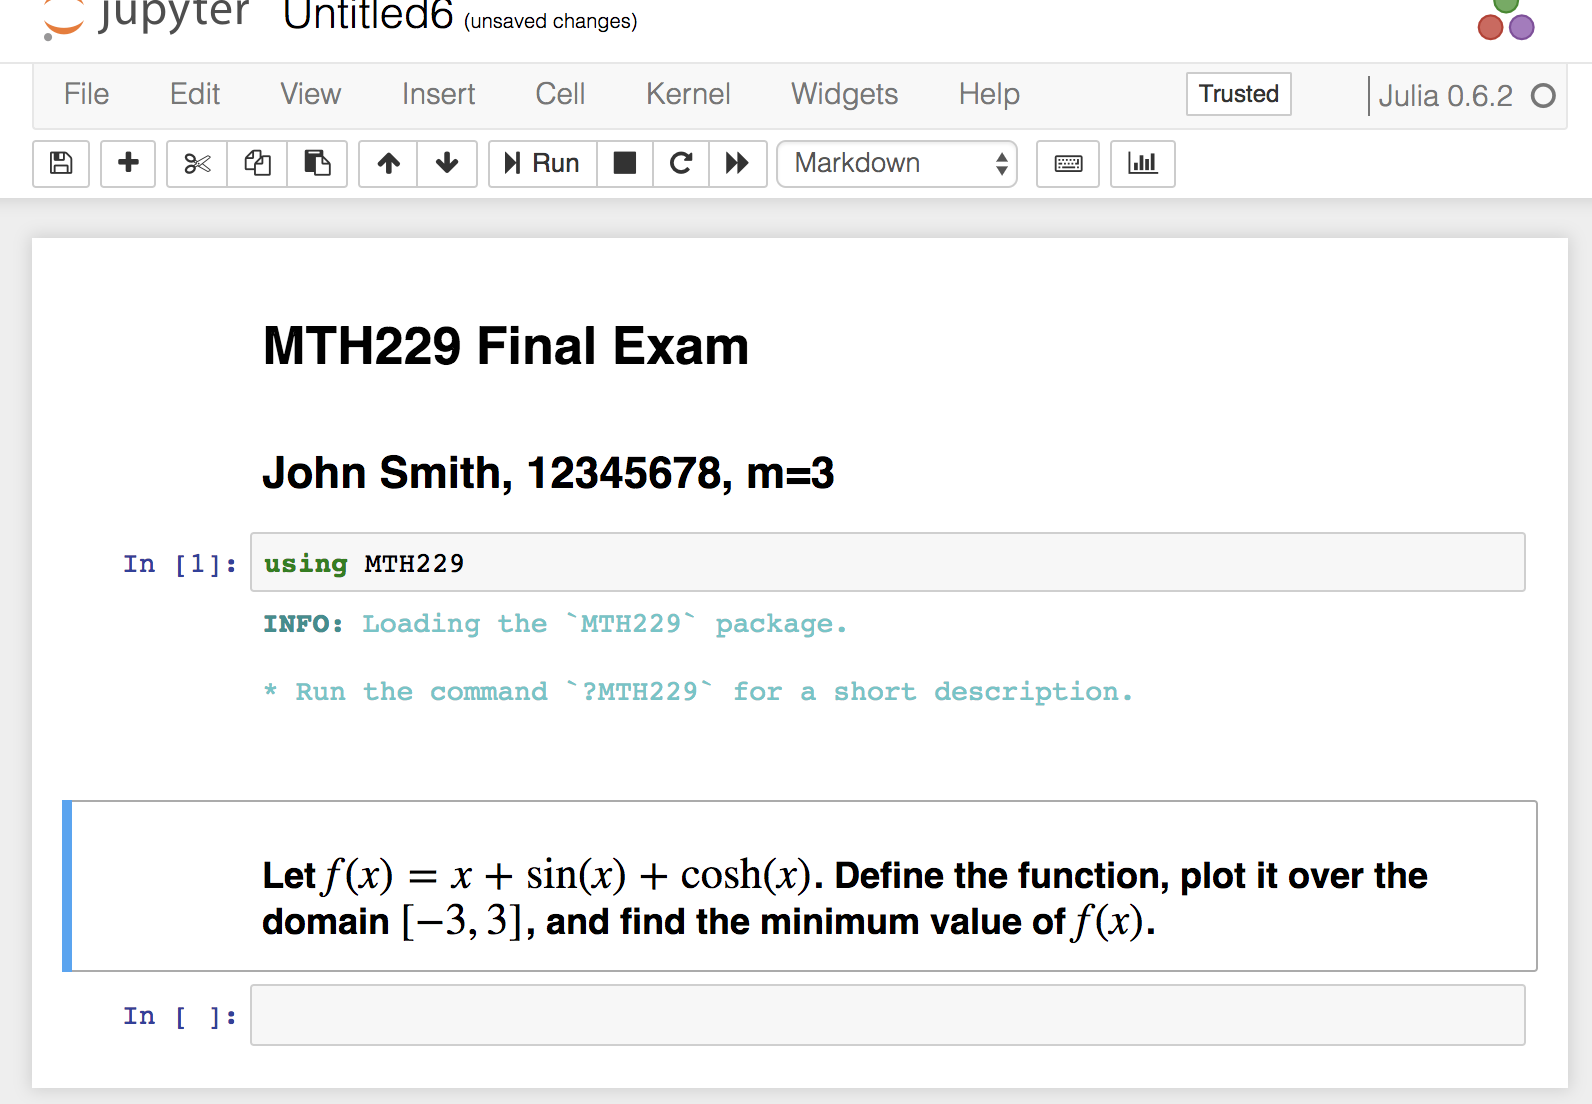
\includegraphics[width=5in]{SkeletonNotes/extracredit-1.png} \end{center}

  \item This is a good  moment to figure out how to save your work (use your name as the  file  name),  and how to locate the {\tt .ipynb} file. Especially if you are using Binder, make sure you have work saved where it won't disappear.

  \item Solve the problem. Don't be shy about creating your own markdown cells (but don't use escape-3 to make them bold) to explain what you are doing, or what you are concluding. Real mathematicians use complete sentences.

  \item In a cell below your solution, enter \begin{verbatim} *** \end{verbatim} and convert the cell to markdown, and then use shift-enter. The cell should turn into a horizontal line running the width of the screen.
  \item Save your work.
  \item {\bf SECOND PROBLEM:} In a new cell, type (replacing $m$ with the value assigned to you).
  \begin{lstlisting}[breaklines]
    Let $$g(x) = \sin(x)\cos(m x)\sin(\pi x).$$ Graph $g$ on the interval $[0,2]$, and also the tangent line at $x=\sqrt{2}$. Compute the roots of $g$ in the interval $[0,2]$. Find the minimum and maximum values of $g$ on $[0,2]$.
  \end{lstlisting}
  Convert the cell to markdown (escape-m), and bold (escape-3), and typeset (shift-enter).

  \item Solve the problem. Don't be shy about creating your own markdown cells to explain what you are doing, and what you have concluded. Below your solution, create a markdown cell with ``{$***$}'', which gives a horizontal line.

  \item {\bf THIRD PROBLEM:}  In a new cell, type (replacing $m$ with the value assigned to you).
  \begin{lstlisting}[breaklines]
    Let $g(x) = \sin(x)\cos(m x)\sin(\pi x)$. Compute $\int_0^{1/\pi} g(x)\,dx$.
  \end{lstlisting}
  Convert the cell to markdown (escape-m), and bold (escape-3), and typeset (shift-enter).

  \item Solve the problem. Don't be shy about creating your own markdown cells to explain what you are doing, and what you have concluded. Below your solution, create a horizontal line. Save your work.


  \item {\bf FOURTH PROBLEM:}  In a new cell, type (replacing $m$ with the value assigned to you).
  \begin{lstlisting}[breaklines]
    Find all solutions to the equation $\sqrt[3]{x} = \frac{x^2}{m} - 229$.
  \end{lstlisting}
  Warning: that's a cube root, not a square root. Convert the cell to markdown (escape-m), and bold (escape-3), and typeset (shift-enter).

  \item Solve the problem.

  \item {\bf BONUS PROBLEM:} In a new cell, type (replacing $m$ with the value assigned to you).
  \begin{lstlisting}[breaklines]
    Let $$r(x) = \frac{m/\pi}{\log(1+ \sqrt m)} \frac{\tan^{-1} x}{x (m+x^2)}.$$ Compute the derivative $r'(x)$ symbolically. Compute $\int_{-1}^1 r(x) \, dx$ numerically. Find estimates for the inflection points of $r(x)$.
  \end{lstlisting}
  Convert the cell to markdown (escape-m), and bold (escape-3), and typeset (shift-enter).
  \item Solve the problem. Don't be shy about creating your own markdown cells to explain what you are doing, and what you have concluded. Below your solution, create a horizontal line. Save your work.

\end{enumerate}

\section{The problems}
\begin{description}
  \item[FIRST:] Let $f(x) = x+4\sin(x)+\cosh(x)$. Define the function, plot it over the domain $[-3,3]$, and find the maximum value of $f(x)$.
  \item[SECOND:] Let $\displaystyle g(x) = \sin(x)\cos(m x)\sin(\pi x).$ Graph $g$ on the interval $[0,2]$, and also the tangent line at $x=\sqrt{2}$. Compute the roots of $g$ in the interval $[0,2]$. Find the minimum and maximum values of $g$ on $[0,2]$.
  \item[THIRD:] Let $g(x) = \sin(x)\cos(m x)\sin(\pi x)$. Compute $\int_0^{1/\pi} g(x)\,dx$.
  \item[FOURTH:] Find all solutions to the equation $\sqrt[3]{x} = \frac{x^2}{m} - 229$.
  \item[BONUS:] Let $\displaystyle r(x) = \frac{m/\pi}{\log(1+ \sqrt m)} \frac{\tan^{-1} x}{x (m+x^2)}.$ Compute the derivative $r'(x)$ symbolically. Compute $\int_{-1}^1 r(x) \, dx$ numerically. Find estimates for the inflection points of $r(x)$.
\end{description}


\end{document}
